%\documentclass[handout,space,nooutcomes]{ximera}
\documentclass{ximera}

\graphicspath{{./}{eulerCharacteristic}}

%\usepackage[strict]{changepage}
\pgfplotsset{compat=1.15}


\title{Spherical Geometry and Beyond}
\author{Brad Findell \and Bart Snapp}
\begin{document}
\begin{abstract}
Here we investigate hyperbolic geometry and compare to Euclidean (flat) geometry and spherical geometry.   
\end{abstract}
\maketitle


%In our approach to Euclidean (i.e., flat) geometry, we make the following assumptions:
%\begin{itemize}
%\item \textbf{(A1)} Through two distinct points passes a unique line.
%\item \textbf{(A2)} Given a line and a point not on the line, there is exactly one line passing through the point which is parallel to the given line (Parallel postulate).
%\item \textbf{(A3)} The points on a line can be placed in one-to-one correspondence with the real numbers so that differences measure distances (Ruler postulate).  
%\item \textbf{(A4)} The rays with a common endpoint can be numbered so that differences measure angles and so that straight angles measure $180^\circ$ (Protractor postulate). 
%\item \textbf{(A5)} Every basic rigid motion (rotation, reflection, or translation) has the following properties:
%\begin{enumerate}
%\item It maps a line to a line, a ray to a ray, and a segment to a segment.
%\item It preserves distance and angle measure.
%\end{enumerate}
%\item \textbf{(A6)} Areas of geometric figures have the following properties: 
%\begin{enumerate}
%\item Congruent figures enclose equal areas.
%\item Area is additive, i.e., the area of the union of two regions that overlap only at their boundaries is the sum of their areas. 
%%\item Area is measured by tiling a region with a two-dimensional unit (such as a square) and parts of the unit, without gaps or overlaps. 
%\item A rectangle with side-lengths $a$ and $b$ has area $ab$, where $a$ and $b$ can be any non-negative real numbers.
%\end{enumerate}
%\end{itemize}


\section*{Getting Started}
Previously, we explored geometry on the (two-dimensional) surface of a sphere and compared it to the two-dimensional Euclidean geometry of a plane.  Both of these geometries have ``constant curvature,'' which is to say the curvature is the same at every point.  Euclidean geometry is flat, and its curvature is 0.  A sphere of radius $R$ has curvature of $1/R^2$.  Thus, all spherical geometries have positive curvature, and a sphere with a very large radius has curvature that is close to $\answer{0}$, which makes sense because a small portion of large sphere is almost flat.  

At this point, an obvious question is, ``Can surfaces have negative curvature?''  The answer is, ``Yes!''  A surface with constant negative curvature is called a \emph{hyperbolic plane}.  In the questions and problems below, we explore hyperbolic geometry and compare it to both spherical and Euclidean geometries.  


%At any point on a surface, we can find a normal vector that is at right angles to the surface; planes containing the normal vector are called normal planes. The intersection of a normal plane and the surface will form a curve called a normal section and the curvature of this curve is the normal curvature. For most points on most “smooth” surfaces, different normal sections will have different curvatures; the maximum and minimum values of these are called the principal curvatures. The Gaussian curvature of a surface is the product of the two principal curvatures.  

\begin{problem}
The GeoGebra sketch below illustrates the principal curvatures at point $P$ on three different surfaces.  The Gaussian curvature of a surface is the product of the two principal curvatures.  
\begin{center}
\geogebra{qgyhqgt9}{702}{354}
\end{center}

For the cylinder, one of the principal curvatures is zero, so its Gaussian curvature is $\answer{0}$.  This makes sense because the cylinder can be flattened on a plan without distortion.  

For the sphere, the principal curvatures go in \wordChoice{\choice[correct]{the same direction}\choice{opposite directions}}, so its Gaussian curvature is positive.  Furthermore, on a sphere the curvature is the same everywhere.  
 
For the hyperbolic paraboloid, the principal curvatures go in \wordChoice{\choice{the same direction}\choice[correct]{opposite directions}}, so its Gaussian curvature is 
negative.  

Side note: The curvature of a hyperbolic paraboloid is most negative at the saddle point and less negative elsewhere, so it cannot serve as a model of a hyperbolic plane, which has \wordChoice{\choice[correct]{constant}\choice{varying}} curvature.  But because the saddle point is much like a Pringles potato chip, it helps to imagine that a hyperbolic plane is like a Pringles potato chip everywhere!  
\end{problem}

\begin{problem}
With constant positive curvature, a sphere curves toward itself and eventually closes to complete a \wordChoice{\choice[correct]{finite}\choice{infinite}} area.  A skull cap can represent a small portion of a sphere, just as a sheet of paper can represent a small portion of a (flat) Euclidean plane.  

With constant negative curvature, a hyperbolic surface curves away from itself and extends infinitely.  Daina Taimina has created crocheted models of portions of hyperbolic planes.  See some pictures \href{https://www.theiff.org/oexhibits/oe1e.html}{here}.  

We explored a disc model of spherical geometry and a Poincare disc model of hyperbolic geometry.  Representing curved surfaces on a flat computer screen requires some distortion.  Both models represent ``straight'' lines with curves, and both models represent angles accurately.  (Other models make different choices.)

In both cases, we saw that as the disc got larger, the angles sums in triangles became closer to $\answer{180}$ degrees, which is to say the models were closer to $\answer[format=string]{Euclidean}$ geometry.  
% And distortion was less?  
\end{problem}

%\section*{Preliminaries}
%
%\begin{problem}
%When studying the geometry of curves and surfaces, we need angles to describe the intersections of curves.   At an intersection point of two smooth curves, the angle between the curves is defined as the angle between \emph{tangents} to the curves.  
%
%Note: Informally, some say that a tangent to a curve touches the curve only once, but this description is misleading.  For example line $k$ is a tangent to a curve $f$ at point $A$, but it intersects the curve again at point $D$.  And what about a tangent to a line?  
%
%\begin{center}
%\definecolor{uuuuuu}{rgb}{0.26666666666666666,0.26666666666666666,0.26666666666666666}
%\definecolor{qqwuqq}{rgb}{0.,0.39215686274509803,0.}
%\begin{tikzpicture}[line cap=round,line join=round,>=triangle 45,x=1.0cm,y=1.0cm]
%\begin{axis}[
%x=1.0cm,y=1.0cm,
%axis lines=middle,
%xmin=-0.8,
%xmax=7.8,
%ymin=-1.1,
%ymax=4.0,
%xtick={0.0,1.0,...,7.0},
%ytick={0.0,1.0,...,3.0},]
%\clip(-0.8,-1.1) rectangle (7.8,3.9);
%\draw[line width=1.pt,color=qqwuqq,smooth,samples=100,domain=-0.8:7.8] plot(\x,{((\x)-1)*((\x)-4)^(2)*((\x)+2)/12});
%\draw [line width=1.pt,domain=-0.8:7.8] plot(\x,{(--0.6666666666666672--0.33333333333333304*\x)/1.});
%\begin{scriptsize}
%\draw [fill=uuuuuu] (2.,1.3333333333333333) circle (1.5pt);
%\draw[color=uuuuuu] (1.86,1.63) node {$A$};
%\draw [fill=uuuuuu] (5.,2.3333333333333335) circle (1.5pt);
%\draw[color=uuuuuu] (5.22,2.15) node {$D$};
%\draw[color=uuuuuu] (4.95,3.5) node {$f$};
%\draw[color=uuuuuu] (7.4,2.9) node {$k$};
%\end{scriptsize}
%\end{axis}
%\end{tikzpicture}
%\end{center}
%
%In calculus, a tangent is defined as a line through two points ``infinitely close’’ to each other on the curve.  Intuitively, we can imagine zooming in close enough so that the curve appears straight.  Then we see that points far away are not relevant.  And it becomes clear that a tangent to a line is the line itself.  
%
%Then, a radius of a circle is perpendicular to the circle because it is perpendicular to the tangent where the radius meets the circle. 
%
%\end{problem}
%
%

\section*{Assumptions}
Euclidean geometry is based on assumptions about fundamental objects, such as points and lines, from which geometry is built. These assumptions are sometimes called postulates or axioms. In the following problems, we consider whether these assumptions hold in hyperbolic geometry. 


\begin{problem} % (A1)
Euclidean assumption: Through two distinct points passes a unique line.  

Does this assumption hold in hyperbolic geometry? 
$\answer[format=string]{yes}$

\begin{feedback}[correct]
\textbf{Correct!}   
\end{feedback}
\end{problem}

\begin{problem} % (A2)
Euclidean assumption: Given a line and a point not on the line, there is exactly one line passing through the point which is parallel to the given line (Parallel postulate).  

Does this assumption hold in hyperbolic geometry? 
$\answer[format=string]{no}$
\begin{problem}
In hyperbolic geometry, there is \wordChoice{\choice{one}\choice{zero}\choice[correct]{more than one}} parallel through a point not on a line. 
\begin{feedback}[correct]
In fact, this is the defining distinction between hyperbolic and Euclidean geometry.  The figure below shows, in a disc model, three different lines through $C$, all parallel to line $\overleftrightarrow{AB}$.  
\begin{center}
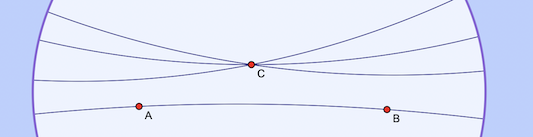
\includegraphics{hyperbolicParallels.png}
\end{center}
Note: In a hyperbolic or Euclidean plane, distinct lines are said to be \emph{parallel} if they do not intersect.  

{\color{red} \emph{Warning:} Lines are sometimes defined as \emph{parallel} when they are the same distance apart.  For hyperbolic geometry, this is not a useful definition.}  
\end{feedback}
\end{problem}
\end{problem}

\begin{problem} % (A3)
Euclidean assumption:  The points on a line can be placed in one-to-one correspondence with the real numbers so that differences measure distances (Ruler postulate).  

Does this assumption hold in hyperbolic geometry? 
$\answer[format=string]{yes}$
\begin{feedback}[correct]
In hyperbolic geometry, lines are \wordChoice{\choice{finite}\choice[correct]{infinite}} in length, so there are no ``wrap-around'' challenges posed by spherical geometry.  
\end{feedback}
\end{problem}

\begin{problem} % (A4)
Euclidean assumption:  The rays with a common endpoint can be numbered so that differences measure angles and so that straight angles measure $180^\circ$ (Protractor postulate).  

Does this assumption hold in hyperbolic geometry? 
$\answer[format=string]{yes}$
\end{problem}

\begin{problem} % (A5)
Euclidean assumption: Every basic rigid motion (rotation, reflection, or translation) has the following properties: 
\begin{enumerate}
\item It maps a line to a line, a ray to a ray, and a segment to a segment.
\item It preserves distance and angle measure.
\end{enumerate}

Does this assumption hold in hyperbolic geometry? 
$\answer[format=string]{yes}$
\begin{feedback}[correct]
\textbf{Correct!} In hyperbolic geometry, translations along a line are challenging to imagine because points off the line cannot move parallel to the line but instead on a ``curve of constant distance from the given line.''  For a good analogy, consider that in spherical geometry, a translation along the equator is a rotation about the axis of the earth, so a point off the equator moves on a curve of constant latitude.
\end{feedback}
\end{problem}

\begin{problem} % A6
Euclidean assumption:  Areas of geometric figures have the following properties: 
\begin{enumerate}
\item Congruent figures enclose equal areas.
\item Area is additive, i.e., the area of the union of two regions that overlap only at their boundaries is the sum of their areas. 
\item A rectangle with side-lengths $a$ and $b$ has area $ab$, where $a$ and $b$ can be any non-negative real numbers.
\end{enumerate}

Does this assumption hold in hyperbolic geometry? 
$\answer[format=string]{no}$
\begin{problem}
Rectangles (i.e., quadrilaterals with four $\answer[format=string]{right}$ angles) do not exist in hyperbolic geometry.    

In Euclidean geometry, area can be based on tiling with unit squares.  But in hyperbolic geometry, squares don't exist, and regular quadrilaterals don't tile the plane, so another approach is needed. 
\end{problem}
\end{problem}

\section*{Problems}

\begin{problem}
\begin{enumerate}
\item In \emph{Euclidean} geometry, the sum of the interior angles of a triangle is 
\wordChoice{\choice{less than}\choice[correct]{equal to}\choice{greater than}} 
$\answer{180}$ degrees.
\item In \emph{spherical} geometry, the sum of the interior angles of a triangle is 
\wordChoice{\choice{less than}\choice{equal to}\choice[correct]{greater than}} 
$\answer{180}$ degrees.
\item In \emph{hyperbolic} geometry, the sum of the interior angles of a triangle is 
\wordChoice{\choice[correct]{less than}\choice{equal to}\choice{greater than}} 
$\answer{180}$ degrees.
\end{enumerate}
\end{problem}

\begin{problem}
\begin{enumerate}
\item In \emph{Euclidean} geometry, the sum of the interior angles of a quadrilateral is 
\wordChoice{\choice{less than}\choice[correct]{equal to}\choice{greater than}} 
$\answer{360}$ degrees.
\item In \emph{spherical} geometry, the sum of the interior angles of a quadrilateral is 
\wordChoice{\choice{less than}\choice{equal to}\choice[correct]{greater than}} 
$\answer{360}$ degrees.
\item In hyperbolic geometry, the sum of the interior angles of a quadrilateral is 
\wordChoice{\choice[correct]{less than}\choice{equal to}\choice{greater than}} 
$\answer{360}$ degrees.
\end{enumerate}
\begin{problem}
In all three geometries, if we draw one $\answer[format=string]{diagonal}$ of the quadrilateral, we divide it into two triangles.  Furthermore, the interior angles of the quadrilateral are made up of interior angles of the two triangles.  The angle sum of a quadrilateral is exactly the sum of the angles of the two triangles.  
\end{problem}
\end{problem}

\begin{problem} % Betweenness
In Euclidean geometry, if three distinct points are collinear, then exactly one must lie between the other two.  Does this statement hold in hyperbolic geometry? 
$\answer[format=string]{yes}$
\begin{feedback}[correct]
In hyperbolic geometry, lines are \wordChoice{\choice{finite}\choice[correct]{infinite}} in length, so there are no ``wrap-around'' challenges posed by spherical geometry.  
\end{feedback}
\end{problem}


%\begin{problem}
%In Euclidean geometry, a rectangle is a quadrilateral with four right angles. 
%\begin{enumerate}
%\item What can you conclude about rectangles in spherical geometries?  Explain.  
%\item What does this imply about the usefulness of familiar (Euclidean) area formulas in these other geometries?  Explain your reasoning. 
%\end{enumerate} 
%\end{problem}

\begin{problem}
In Euclidean geometry, given a line and a point, there is a unique perpendicular to the given line through the given point.  In hyperbolic geometry, to what extent is this true? 
\begin{multipleChoice}
\choice[correct]{Always.}
\choice{Sometimes.}
\choice{Never.}
\end{multipleChoice}
\begin{problem}
Correct!  Here are two arguments across the three geometries. 

First, two distinct perpendiculars from a given point to a given line would create a triangle with an angle sum 
\wordChoice{\choice{less than}\choice{equal to}\choice[correct]{greater than}} $\answer{180}$ degrees.  
\begin{itemize}
\item In hyperbolic geometry, such a triangle \wordChoice{\choice{can}\choice[correct]{cannot}} exist because \emph{every} triangle has an angle sum less than $180^\circ$.  
\item In Euclidean geometry, such a triangle \wordChoice{\choice{can}\choice[correct]{cannot}} exist because \emph{every} triangle has an angle sum equal to $180^\circ$.  
\item In spherical geometry, such a triangle \wordChoice{\choice[correct]{can}\choice{cannot}} exist because \emph{every} triangle has an angle sum greater than $180^\circ$.  
\end{itemize}

\begin{center}
\definecolor{qqwuqq}{rgb}{0.,0.39215686274509803,0.}
\begin{tikzpicture}[line cap=round,line join=round,>=triangle 45,x=1.0cm,y=1.0cm,scale=0.7]
\clip(-3.,-0.1) rectangle (12.,2.1);
\draw[line width=1.pt,color=qqwuqq,fill=qqwuqq,fill opacity=0.10000000149011612] (11.213940785051445,1.5646044445518976) -- (11.21815649207423,1.3137815882398602) -- (11.468979348386268,1.3179972952626449) -- (11.464763641363483,1.5688201515746822) -- cycle; 
\draw[line width=1.pt,color=qqwuqq,fill=qqwuqq,fill opacity=0.10000000149011612] (11.461786817329786,0.7195226672674778) -- (11.211000291969182,0.7255223449076836) -- (11.205000614328977,0.4747358195470804) -- (11.45578713968958,0.46873614190687457) -- cycle; 
\draw [line width=1.pt] (-1.564168514412414,1.1250554323725062) circle (13.036487266354374cm);
\draw [line width=1.pt] (10.506146939582424,-161.7727998905248) circle (163.34443297510484cm);
\draw [line width=1.pt] (10.290942751443046,106.83278616774713) circle (106.37042822301825cm);
\end{tikzpicture}
\end{center}

\begin{problem}
Second, consider any two distinct perpendiculars to a given line.  
\begin{itemize}
\item In hyperbolic geometry, the two perpendiculars \wordChoice{\choice[correct]{must be}\choice{might be}\choice{cannot be}} parallel.    
\item In Euclidean geometry, the two perpendiculars \wordChoice{\choice[correct]{must be}\choice{might be}\choice{cannot be}} parallel.  
\item In spherical geometry, the two perpendiculars \wordChoice{\choice{must be}\choice{might be}\choice[correct]{cannot be}} parallel 
\end{itemize}
\begin{problem}
Correct!  In $\answer[format=string]{spherical}$ geometry, parallel lines don't exist!   

Furthermore:  
\begin{itemize}
\item In $\answer[format=string]{hyperbolic}$ geometry, the two perpendiculars grow further apart away from the intersections with the given line.  
\begin{center}
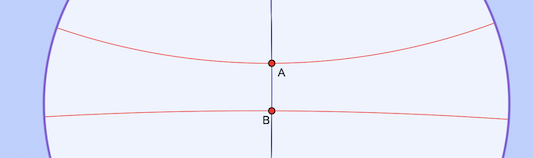
\includegraphics{hyperbolicPerpendiculars.png}
\end{center}
\item In $\answer[format=string]{Euclidean}$ geometry, the two perpendiculars are always the same distance apart away from the intersections with the given line.  
\begin{center}

\includegraphics{euclideanPerpendiculars.png}
\end{center}
\item In $\answer[format=string]{spherical}$ geometry, the two perpendiculars become closer together away from the intersections with the given line. In fact, the two perpendiculars intersect at two points on opposite ends of a diameter of the sphere. 
\begin{center}
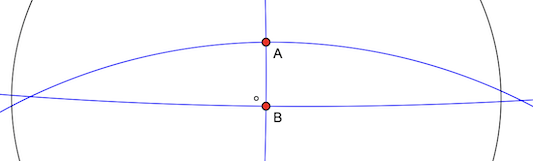
\includegraphics{sphericalPerpendiculars.png}
\end{center}
\end{itemize}
\end{problem}
\end{problem}
\end{problem} 
\end{problem}

\begin{problem}
Can the Euclidean definition of a circle make sense on the hyperbolic plane?  
\begin{multipleChoice}
\choice[correct]{Yes.}
\choice{Yes, with some adjustments in interpretation.}
\choice{No.}
\end{multipleChoice}
\begin{problem}
Correct! And no adjustments in interpretation are needed.

Here is the definition:  

A circle is the set of points that are $\answer[format=string]{equidistant}$ from a given point, called the $\answer[format=string]{center}$ of the circle.  The common distance is called the $\answer[format=string]{radius}$ of the circle.  

In the disc model, the center of a circle might not appear to be the center, but that is because the model distorts distances.  

\begin{problem}
Will the Euclidean circumference and area formulas hold?  
$\answer[format=string]{no}$. 
\begin{problem}
On a Euclidean plane, the circumference of a circle of radius $r$ is $\answer{2\pi r}$, and its area is $\answer{\pi r^2}$.  Hint: Use pi for $\pi$. 

On a sphere, moving away from the center of the circle, the surface curves \wordChoice{\choice[correct]{toward}\choice{away from}} itself, which creates \wordChoice{\choice[correct]{less}\choice{the same}\choice{more}} circumference than on a Euclidean plane as well as \wordChoice{\choice[correct]{less}\choice{the same}\choice{more}} area than on a Euclidean plane.  

On a hyperbolic plane, moving away from the center of the circle, the surface curves \wordChoice{\choice{toward}\choice[correct]{away from}} itself, which creates \wordChoice{\choice{less}\choice{the same}\choice[correct]{more}} circumference than on a Euclidean plane as well as \wordChoice{\choice{less}\choice{the same}\choice[correct]{more}} area than on a Euclidean plane.  
\begin{feedback}[correct]
Correct!  This is why crocheted models of the hyperbolic plane are so ``leafy,'' with much extra area.  
\end{feedback}

\end{problem}
\end{problem}
\end{problem}
\end{problem}





\end{document}
